\input{configuration}

\title{Lecture 33 --- Parallel Databases }

\author{Jeff Zarnett \\ \small \texttt{jzarnett@uwaterloo.ca}}
\institute{Department of Electrical and Computer Engineering \\
  University of Waterloo}
\date{\today}


\begin{document}

\begin{frame}
  \titlepage

 \end{frame}
 
 

\begin{frame}
\frametitle{Concurrency and Parallelism}

How do we implement the server?

If each incoming transaction to be processes is assigned a thread, then we could have $n$ worker threads and a transaction gets picked up by a worker. 

Keeping in mind that locking and coordination are needed, but the maximum theoretical speedup is limited by the number of processors.

\begin{center}
	
\includegraphics[width=0.3\textwidth]{images/familiar.jpg}
\end{center}


Or a pipeline architecture?
\end{frame}
 
 


\begin{frame}
\frametitle{I/O Parallelism}

If the database is aware of the various disks available in the system, we can speed up performance via I/O parallelism. 

To read some blocks from disk, we could let multiple requests run in parallel. 

If there are three blocks we need, and three disks, we could get all three results at (roughly) the same time. 

\end{frame}


\begin{frame}
\frametitle{I/O Parallelism: Disk Partitioning}

We'll consider three basic partitioning strategies assuming we have $n$ disks:
\begin{itemize}
	\item \textbf{Round-Robin}
	\item \textbf{Hash Partitioning}
	\item \textbf{Range Partitioning}
\end{itemize}

\end{frame}


\begin{frame}
\frametitle{I/O Parallelism}

There are three operations we consider likely to happen:

(1) Scanning the entire relation; 

(2) Locating a tuple with some specific attribute equal to a certain value, and 

(3) Range queries (where we have a range of acceptable values of the attribute).

\end{frame}

\begin{frame}
\frametitle{Round Robin}

Round Robin is good for when we have to read the whole relation. 

\begin{center}
	
\includegraphics[width=0.25\textwidth]{images/rr.jpg}
\end{center}

But no advantage is gained when a specific query or range query is done as we have to search over everything anyway.

\end{frame}

\begin{frame}
\frametitle{Hash Partitioning}

Hash partitioning is advantageous when we do specific queries. 

This is only beneficial, of course, if the items are partitioned based on that particular attribute. 

\begin{center}
	
\includegraphics[width=0.3\textwidth]{images/hashbrown.jpg}
\end{center}

\end{frame}

\begin{frame}
\frametitle{Hash Partitioning}
In theory it search time could be reduced to $1/n$ of the original time. 

Otherwise no advantage is gained over round robin. 

This is also not especially suitable for range queries.

\end{frame}

\begin{frame}
\frametitle{Range Partitioning}

Range partitioning is good for specific as well as range queries on a particular attribute. 

A nice advantage of this is if we know that a query will be only on one disk, it's possible to send the query to just one disk.

The other disks are available to perform other operations.


\end{frame}

\begin{frame}
\frametitle{Skew}

When the relation is spread over several disks, if things are not spread out evenly, then there is \alert{skew} in the distribution of tuples. 


This can be because of either \alert{attribute-value} skew: city = ``Toronto'' being much more common than ``Yellowknife'', for example.

Or it can be because of the way the partitioning function works even if values are evenly distributed.
\end{frame}


\begin{frame}
\frametitle{Balancing Skew}

To balance this out, one suggested strategy is the histogram approach. 

Suppose there are, for example, 5 disks and 100 possible values. 

The simple range approach is 20 values in each partition. 

If the data has a normal distribution however... Rather than 20 values per disk we would try to cut it so there are about 20\% of tuples in each partition.

\end{frame}


\begin{frame}
\frametitle{Slice and Dice!}

An alternative approach is to cut it all up more. More?

\begin{center}
	
\includegraphics[width=0.5\textwidth]{images/more.jpg}
\end{center}

Suppose there are $n$ processors and the work is divided up into $5n$ ranges. 

If the data is evenly distributed, each CPU will do 5 chunks. 

\end{frame}


\begin{frame}
\frametitle{Slice and Dice!}

If the work is unevenly divided, however, some CPUs will do a smaller number of large chunks.

Others will do a large number of smaller chunks and some will be in between. 

The uneven distribution of values is then spread out over several processors. 


\end{frame}

\begin{frame}
\frametitle{Realistic? Maybe...}

Admittedly, in a single server database this is not likely to happen even when there are multiple disks. 

Usually the disks are arranged in a RAID array and that is done outside the purview of the database server... 

So why did we learn about this? \\
\quad Because it will be useful in a distributed database.

\end{frame}


\begin{frame}
\frametitle{Intraquery Parallelism}

The subject of inter-query parallelism is actually somewhat boring and redundant.

It is just the same as previous discussions of parallelism and concurrency. 

Lock shared data, you know the drill. 

\begin{center}
	
\includegraphics[width=0.4\textwidth]{images/notagain.jpg}
\end{center}

\end{frame}


\begin{frame}
\frametitle{Intraquery Parallelism}

But there are numerous opportunities to get parallelism inside a single query, and it is a much more interesting subject. 

We'll consider: intraoperation parallelism and interoperation parallelism.

\end{frame}



\begin{frame}
\frametitle{Intraoperation Parallelism}

When we have a single operation that can be, in some way, divided up (partitioned) it is a good candidate for intraoperation parallelism. 

\begin{itemize}
	\item Searching
	\item Sorting
	\item Calculation
\end{itemize}

\end{frame}

\begin{frame}
\frametitle{Partitioned Join}

Example: parallel join, in particular a partitioned join. 

Let's assume we want to join relations $r$ and $s$. 

If the join is an equality condition such as one attribute in $r$ equalling another in $s$ then we can divide this up to multiple processors.

\end{frame}

\begin{frame}
\frametitle{Partitioned Join}
If there are $n$ processors we could divide each relation into $n$ pieces and send each processor $P_{i}$ its piece of $r$ and $s$. 

That processor then compute its part. 

These parts are then combined at the end to produce the correct data. 


\end{frame}

\begin{frame}
\frametitle{Partitioned Parallel Join}

\begin{center}
\includegraphics[width=0.7\textwidth]{images/partitioned-parallel-join}
\end{center}

\end{frame}

\begin{frame}
\frametitle{Fragment and Replicate}

Partitioning is not suitable for all types of joins, however; because we put in the restriction that there is a join on an equality condition. 

A more general approach is the \alert{asymmetric fragment-and-replicate join}.

\end{frame}

\begin{frame}
\frametitle{Fragment and Replicate}

\begin{enumerate}
\item Partition one of the relations ($r$) and hand out the partitions to the processors.
\item Send copies of the whole other relation ($s$) to every processor.
\item Each processor computers its join (through whatever method) and the data is recombined. 
\end{enumerate}

It would be preferable to choose the smaller relation to be the one that is copied.

\end{frame}

\begin{frame}
\frametitle{Fragment and Replicate}

\begin{center}
\includegraphics[width=0.85\textwidth]{images/fragment-and-replicate}
\end{center}

\end{frame}


\begin{frame}
\frametitle{Parallelism Roundup}

How parallelism affects operations other than selection and join:
\begin{itemize}
\item \textbf{Duplicate Elimination}
\item \textbf{Projection}
\item \textbf{Aggregation}
\end{itemize}

\end{frame}

\begin{frame}
\frametitle{Interoperation Parallelism }

We already discussed the idea of pipelining.

This, unfortunately, does not scale well: a pipeline with 4 stages cannot really take advantage of 16 processors.

The next way that we can use parallelism between various operations. 

If we are to join four tables, we could compute two pairs of joins in parallel and then combine them in a third operation for the last step. 

\end{frame}



\begin{frame}
\frametitle{Change is Hard}

We would normally expect that when changes are made to the database schema such as data migration, the database is taken temporarily off the line.

Sometimes we don't have the option to take things offline for a long period.

\end{frame}

\begin{frame}
\frametitle{Change is Hard}

If a new index is to be built we can't just lock the relation in shared mode.

We have to allow insertion, deletion, and update while the index is being added. 

\end{frame}

\begin{frame}
\frametitle{Change is Hard}

This is usually done by just keeping track of all the changes as they come in.

\begin{center}
	
\includegraphics[width=0.5\textwidth]{images/pileup.jpg}
\end{center}

Then, adjust the index when generated to account for all the changes that happened while it was being built.

\end{frame}

\begin{frame}
\frametitle{Parallel Database Architecture}

Now if we have a parallel database, we should consider the architecture. 


Three possible options: shared memory, shared disk, and shared nothing.


\end{frame}

\begin{frame}
\frametitle{Shared Memory}

This is our typical multicore or multi-CPU architecture we have likely already become familiar with when discussing concurrency. 

Memory is shared between the various processors; they have common disks. 

There is no redundancy, however, as it is all wrapped up into one machine.

Communication can take place between the threads using shared memory.

\end{frame}

\begin{frame}
\frametitle{Shared Disk}

In this architecture all processors can access disks directly, but every processor has its own memory. 

This has some degree of redundancy as we might be able to keep working if something goes wrong at one of the systems. 

If one of the systems crashes, every system can continue executing without any problem, at some reduced performance level. 

The tradeoff is that communication has to take place using the disk.

\end{frame}

\begin{frame}
\frametitle{Shared Nothing}

In a shared nothing system, well, it's exactly what it sounds like: nothing is shared between the systems. 

\begin{center}
	
\includegraphics[width=0.3\textwidth]{images/sharefood.jpg}
\end{center}

If they wish to communicate, then it takes place over the network. 

This means the systems are as redundant as possible: if any one system goes down we might be able to carry on. 

\end{frame}

\begin{frame}
\frametitle{Shared Nothing}

This sort of architecture isn't so much parallel as it actually is \alert{distributed}...

\begin{center}
	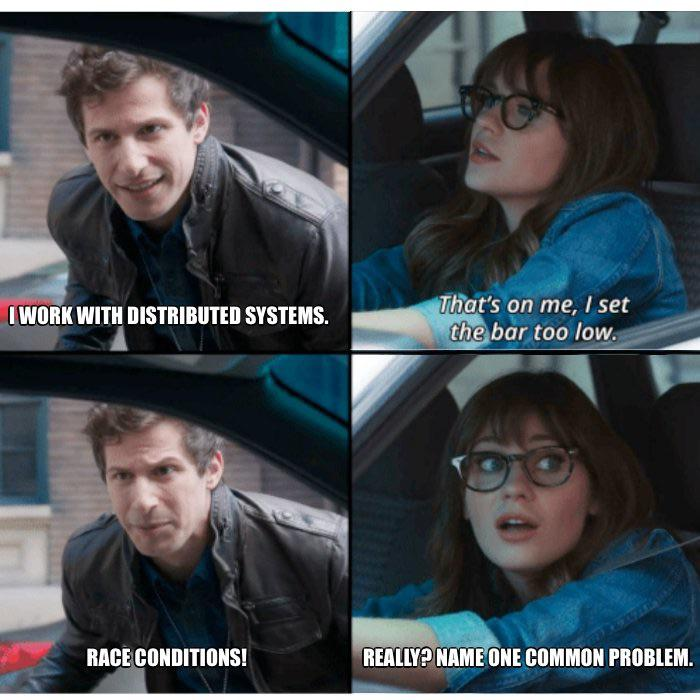
\includegraphics[width=0.6\textwidth]{images/distributed.jpg}
\end{center}


\end{frame}


\end{document}

